\chapter{1 Samuel 15}

\begin{figure}
  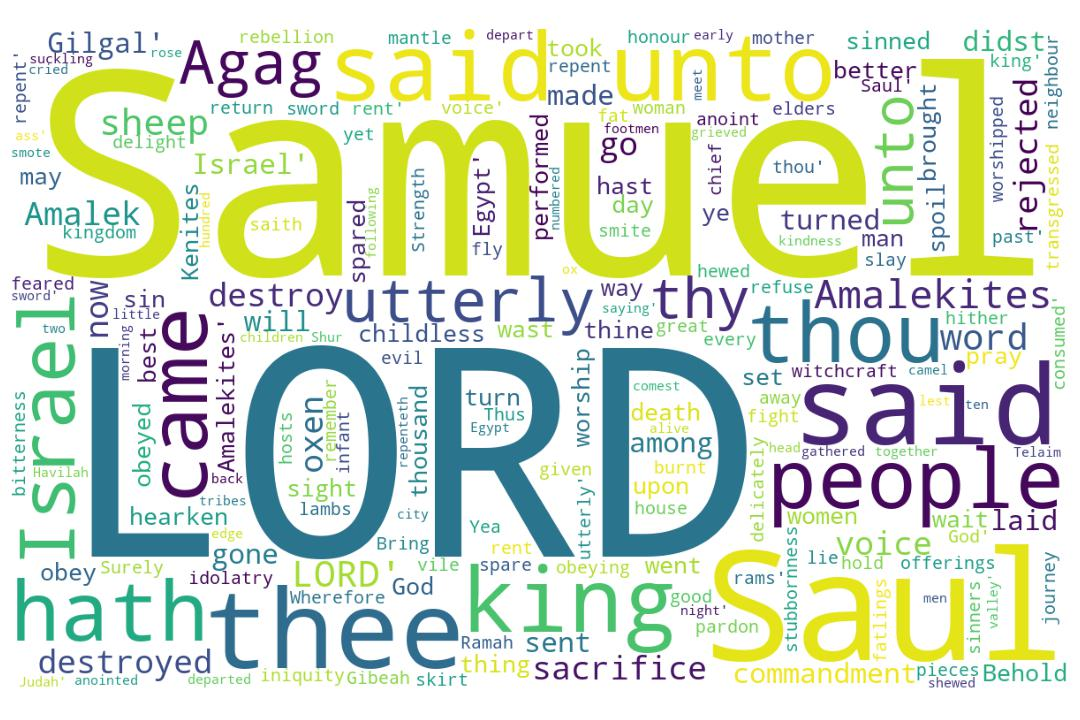
\includegraphics[width=\linewidth]{09OT-1Samuel/1Samuel15-WordCloud.jpg}
  \caption{1 Samuel 15 Word Cloud}
  \label{fig:1 Samuel 15 Word Cloud}
\end{figure}

%%%%%%%%%%%%%%%%%%%%%%%%%%%%%%%%%%%%%%
%%%%%%%%%%%%%%%%%%%%%%%%%%%%%%%%%%%%%%
\marginpar{\scriptsize \centering \fcolorbox{black}{lime}{\textbf{A FAILED TEST}}\\ (1 Samuel 15:1--35) \begin{compactenum}[I.][8]
    \item \textbf{Specific Instructions} \index[scripture]{1Samuel!1Sa 15:03} 1Sa 15:3) 
    \item \textbf{Serious Intransigence} \index[scripture]{1Samuel!1Sa 15:09} (1Sa 15:9) 
    \item \textbf{Selective} \index[scripture]{1Samuel!1Sa 15:13} (1Sa 15:13) 
    \item \textbf{Stubbornness and Iniquity} \index[scripture]{1Samuel!1Sa 15:23} (1Sa15:23) 
    \item The \textbf{Standard and Imperative} \index[scripture]{1Samuel!1Sa 15:23} (1Sa 15:23) 
    \item The \textbf{Strength of Israel} \index[scripture]{1Samuel!1Sa 15:29} (1Sa 15:29) 
    \item \textbf{Certain Indictment} \index[scripture]{1Samuel!1Sa 15:33} (1Sa 15:33) 
\end{compactenum}}

%%%%%%%%%%%%%%%%%%%%%%%%%%%%%%%%%%%%%%
%%%%%%%%%%%%%%%%%%%%%%%%%%%%%%%%%%%%%%
\footnote{\textcolor[cmyk]{0.99998,1,0,0}{\hyperlink{TOC}{Return to end of Table of Contents.}}}\footnote{\href{https://audiobible.com/bible/1_samuel_15.html}{\textcolor[cmyk]{0.99998,1,0,0}{1 Samuel 15 Audio}}}\textcolor[cmyk]{0.99998,1,0,0}{Samuel also said unto Saul, The LORD sent me to anoint thee \emph{to} \emph{be} king over his people, over Israel: now therefore hearken thou unto the voice of the words of the LORD.}
[2] \textcolor[cmyk]{0.99998,1,0,0}{Thus saith the LORD of hosts, I remember \emph{that} which Amalek did to Israel, how \fcolorbox{bone}{bone}{he} laid \emph{wait} for him in the way, when \fcolorbox{bone}{bone}{he} came up from Egypt.}
[3] \textcolor[cmyk]{0.99998,1,0,0}{Now \fcolorbox{black}{lime}{go and smite} Amalek, and utterly destroy all that they \fcolorbox{bone}{bone}{have} , and spare them not; but slay both man and woman, infant and suckling, ox and sheep, camel and ass.}
[4] \textcolor[cmyk]{0.99998,1,0,0}{And Saul gathered the people together, and numbered them in Telaim, two hundred thousand footmen, and ten thousand men of Judah.}
[5] \textcolor[cmyk]{0.99998,1,0,0}{And Saul came to a city of Amalek, and laid wait in the valley.}\\
\\
\P \textcolor[cmyk]{0.99998,1,0,0}{And Saul said unto the Kenites, Go, depart, get you down from among the Amalekites, lest I destroy you with them: for ye shewed kindness to all the children of Israel, when they came up out of Egypt. So the Kenites departed from among the Amalekites.}
[7] \textcolor[cmyk]{0.99998,1,0,0}{And Saul smote the Amalekites from Havilah \emph{until} thou comest to Shur, that \emph{is} over against Egypt.}
[8] \textcolor[cmyk]{0.99998,1,0,0}{And \fcolorbox{bone}{bone}{he} took Agag the king of the Amalekites alive, and utterly destroyed all the people with the edge of the sword.}
[9] \textcolor[cmyk]{0.99998,1,0,0}{But Saul and the people \fcolorbox{black}{lime}{spared Agag}, and the best of the sheep, and of the oxen, and of the fatlings, and the lambs, and all \emph{that} \emph{was} good, and would not utterly destroy them: but every thing \emph{that} \emph{was} vile and refuse, that they destroyed utterly.}\\
\\
\P \textcolor[cmyk]{0.99998,1,0,0}{Then came the word of the LORD unto Samuel, saying,}
[11] \textcolor[cmyk]{0.99998,1,0,0}{It repenteth me that I \fcolorbox{bone}{bone}{have}  set up Saul \emph{to} \emph{be} king: for \fcolorbox{bone}{bone}{he} is turned back from following me, and hath not performed my commandments. And it grieved Samuel; and \fcolorbox{bone}{bone}{he} cried unto the LORD all night.}
[12] \textcolor[cmyk]{0.99998,1,0,0}{And when Samuel rose early to meet Saul in the morning, it was told Samuel, saying, Saul came to Carmel, and, behold, \fcolorbox{bone}{bone}{he} set him up a place, and is gone about, and passed on, and gone down to Gilgal.}
[13] \textcolor[cmyk]{0.99998,1,0,0}{And Samuel came to Saul: and Saul said unto him, Blessed \emph{be} thou of the LORD: I \fcolorbox{black}{lime}{have performed} the commandment of the LORD.}
[14] \textcolor[cmyk]{0.99998,1,0,0}{And Samuel said, What \emph{meaneth} then this bleating of the sheep in mine ears, and the lowing of the oxen which I hear?}
[15] \textcolor[cmyk]{0.99998,1,0,0}{And Saul said, They \fcolorbox{bone}{bone}{have}  brought them from the Amalekites: for the people spared the best of the sheep and of the oxen, to sacrifice unto the LORD thy God; and the rest we \fcolorbox{bone}{bone}{have}  utterly destroyed.}
[16] \textcolor[cmyk]{0.99998,1,0,0}{Then Samuel said unto Saul, Stay, and I will tell thee what the LORD hath said to me this night. And \fcolorbox{bone}{bone}{he} said unto him, Say on.}
[17] \textcolor[cmyk]{0.99998,1,0,0}{And Samuel said, When thou \emph{wast} little in thine own sight, \emph{wast} thou not \emph{made} the head of the tribes of Israel, and the LORD anointed thee king over Israel?}
[18] \textcolor[cmyk]{0.99998,1,0,0}{And the LORD sent thee on a journey, and said, Go and utterly destroy the sinners the Amalekites, and fight against them until they be consumed.}
[19] \textcolor[cmyk]{0.99998,1,0,0}{Wherefore then didst thou not obey the voice of the LORD, but didst fly upon the spoil, and didst evil in the sight of the LORD?}
[20] \textcolor[cmyk]{0.99998,1,0,0}{And Saul said unto Samuel, Yea, I \fcolorbox{bone}{bone}{have}  obeyed the voice of the LORD, and \fcolorbox{bone}{bone}{have}  gone the way which the LORD sent me, and \fcolorbox{bone}{bone}{have}  brought Agag the king of Amalek, and \fcolorbox{bone}{bone}{have}  utterly destroyed the Amalekites.}
[21] \textcolor[cmyk]{0.99998,1,0,0}{But the people took of the spoil, sheep and oxen, the chief of the things which should \fcolorbox{bone}{bone}{have}  been utterly destroyed, to sacrifice unto the LORD thy God in Gilgal.}
[22] \textcolor[cmyk]{0.99998,1,0,0}{And Samuel said, Hath the LORD \emph{as} \emph{great} delight in burnt offerings and sacrifices, as in obeying the voice of the LORD? Behold, to obey \emph{is} better than sacrifice, \emph{and} to hearken than the fat of rams.}
[23] \textcolor[cmyk]{0.99998,1,0,0}{For rebellion \emph{is} \emph{as} the sin of witchcraft, and \fcolorbox{black}{lime}{stubbornness} \emph{is} \emph{as} \fcolorbox{black}{lime}{iniquity} and \fcolorbox{black}{lime}{idolatry}. Because thou hast rejected the word of the LORD, \fcolorbox{bone}{bone}{he} hath also rejected thee from \emph{being} king.}\\
\\
\P \textcolor[cmyk]{0.99998,1,0,0}{And Saul said unto Samuel, I \fcolorbox{bone}{bone}{have}  sinned: for I \fcolorbox{bone}{bone}{have}  transgressed the commandment of the LORD, and thy words: because I feared the people, and obeyed their voice.}
[25] \textcolor[cmyk]{0.99998,1,0,0}{Now therefore, I pray thee, pardon my sin, and turn again with me, that I may worship the LORD.}
[26] \textcolor[cmyk]{0.99998,1,0,0}{And Samuel said unto Saul, I will not return with thee: for thou hast rejected the word of the LORD, and the LORD hath rejected thee from being king over Israel.}
[27] \textcolor[cmyk]{0.99998,1,0,0}{And as Samuel turned about to go away, \fcolorbox{bone}{bone}{he} laid hold upon the skirt of his mantle, and it rent.}
[28] \textcolor[cmyk]{0.99998,1,0,0}{And Samuel said unto him, The LORD hath rent the kingdom of Israel from thee this day, and hath given it to a neighbour of thine, \emph{that} \emph{is} better than thou.}
[29] \textcolor[cmyk]{0.99998,1,0,0}{And also the \fcolorbox{black}{lime}{Strength of Israel} will not lie nor repent: for \fcolorbox{bone}{bone}{he} \emph{is} not a man, that \fcolorbox{bone}{bone}{he} should repent.}
[30] \textcolor[cmyk]{0.99998,1,0,0}{Then \fcolorbox{bone}{bone}{he} said, I \fcolorbox{bone}{bone}{have}  sinned: \emph{yet} honour me now, I pray thee, before the elders of my people, and before Israel, and turn again with me, that I may worship the LORD thy God.}
[31] \textcolor[cmyk]{0.99998,1,0,0}{So Samuel turned again after Saul; and Saul worshipped the LORD.}\\
\\
\P \textcolor[cmyk]{0.99998,1,0,0}{Then said Samuel, Bring ye hither to me Agag the king of the Amalekites. And Agag came unto him delicately. And Agag said, Surely the bitterness of death is past.}
[33] \textcolor[cmyk]{0.99998,1,0,0}{And Samuel said, As thy sword hath made women childless, \fcolorbox{black}{lime}{so shall thy mother be childless} among women. And Samuel hewed Agag in pieces before the LORD in Gilgal.}\\
\\
\P \textcolor[cmyk]{0.99998,1,0,0}{Then Samuel went to Ramah; and Saul went up to his house to Gibeah of Saul.}
[35] \textcolor[cmyk]{0.99998,1,0,0}{And Samuel came no more to see Saul until the day of his death: nevertheless Samuel mourned for Saul: and the LORD repented that \fcolorbox{bone}{bone}{he} had made Saul king over Israel.}